

\section{Protocolos de Roteamento e Topologia}

\begin{frame}{Desafio dos Caminhos e Múltiplos Saltos}
    Os protocolos de roteamento ocorrem dentro da Camada de Rede, que é responsável pelo roteamento de pacote de dados através da rede de sensores. Um problema que essas redes enfrentam é a bateria, pois o consumo de energia usada na comunicação é maior que a utilizada na coleta e processamento de dados, principalmente nas arquiteturas de “salto único” (\textit{single-hop}), onde cada sensor envia os dados diretamente para a estação base. 

    
    Para resolver esse problema, utiliza-se uma arquitetura de “múltiplos saltos” (\textit{multi-hop}) onde cada nó sensor transmite os dados para o nó mais próximo, intermediando a comunicação até chegar na estação base. Como cada nó precisa realizar transmissões de curtas distâncias, essa arquitetura reduz o consumo de energia e aumenta a durabilidade da rede, principalmente quando os nós estão distribuídos em grandes áreas.
\end{frame}

\begin{frame}{Topologias}
    A topologia de uma RSSF define como será o sistema de comunicação entre os sensores, adotando uma de três abordagens: estrela, árvore ou \textit{cluster} e malha.
\end{frame}

\begin{frame}{Estrela}
    A estrela é a mais simples, onde cada nó transmite diretamente para um gateway ou receptor. Essa topologia, entretanto, é limitada pela distância, visto que os nós precisam estar no alcance do \textit{gateway}.
\end{frame}

\begin{frame}{Árvore (Cluster)}
    A topologia árvore (ou \textit{cluster}) permite a extensão dessas distâncias, uma vez que possibilita que cada nó se comunique com nós roteadores, nos quais são capazes de receber dados e não apenas enviá-los. Porém, um problema dessa topologia é que caso um nó roteador perca a comunicação, a sub-rede responsável por enviar dados ao nó perde a comunicação com o \textit{gateway}.
\end{frame}

\begin{frame}{Malha}
    A topologia de malha resolve esse problema ao implementar uma redundância nas rotas de comunicação, onde cada nó pode se comunicar com os demais. Entretanto, essa abordagem é mais custosa pelo fato de que todos os nós devem ter a capacidade de receber e transmitir dados. Além disso, essa abordagem tem um aumento significativo na latência da rede, visto que as rotas exigem mais saltos até chegarem no gateway.
\end{frame}

\begin{frame}{Topologias (Ilustração)}
    \begin{figure}
        \centering
        \caption{Topologias de Redes de Sensores Sem Fio}
        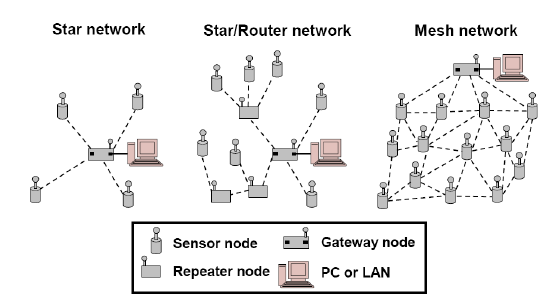
\includegraphics[width=0.65\linewidth]{figuras/topologias.png} 
        \label{fig:topologias}
        \\ \small Fonte: GTA/UFRJ (2018).
    \end{figure}
\end{frame}

\begin{frame}{Roteamento Hierárquico}
    Um algoritmo altamente usado nas RSSFs é o LEACH (\textit{Low-Energy Adaptive Clustering Hierarchy}), aplicado com base na topologia árvore/\textit{cluster}. Usando esse conceito, os nós sensores são segmentados em grupos menores onde cada grupo tem um nó líder ou nó principal, que recebe os dados dos outros sensores e faz a comunicação com a estação-base.
\end{frame}

\begin{frame}{Roteamento Hierárquico (Continuação)}
    Antes da transmissão, o nó líder (também chamado de \textit{cluster-head}) faz um pré-processamento para decidir se haverá agregação dos dados, assim economizando no número de transmissões e gastando menos energia. Este nó também garante o controle de transmissões, permitindo que apenas um nó sensor seja ligado para transmissão por vez.

    
    Neste protocolo, os líderes não são fixos. Na fase de inicialização, cada nó transmite sua energia disponível e sua localização para a estação-base, na qual irá definir os \textit{clusters} e o nó líder, que é escolhido dentre os nós com maior energia restante.
\end{frame}

\begin{frame}{Roteamento Hierárquico (Ilustração)}
    \begin{figure}
        \centering
        \caption{Roteamento Hierárquico}
        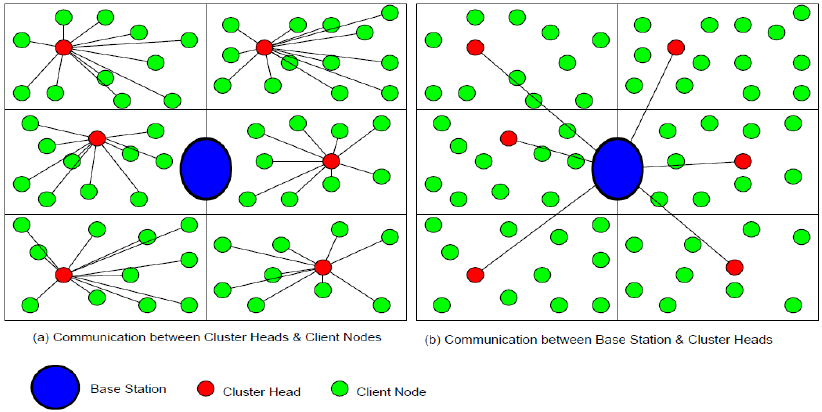
\includegraphics[width=0.7\linewidth]{figuras/roteamento hierarquico.png} 
        \label{fig:roteamento hierarquico}
        \\ \small Fonte: GTA/UFRJ (2018).
    \end{figure}
\end{frame}

\begin{frame}{Roteamento Orientado a Dados}
    Um outro protocolo também usado é o \textit{Directed Diffusion}, no qual seu roteamento se baseia unicamente em dados, não na hierarquia ou em endereços específicos. Nessa abordagem, a comunicação é estabelecida através do nome ou tipo de dado que deseja obter, onde um nó “sorvedouro” (\textit{sink}) solicita uma informação específica denominada “interesse”. Este interesse é difundido (\textit{broadcast}) pela rede até encontrar sensores que contenham tal informação.
\end{frame}

\begin{frame}{Roteamento Orientado a Dados (Continuação)}
    Quando um nó recebe o interesse de um vizinho, ele cria uma rota chamada “gradiente” em seu cache local, que indica a direção para onde os dados correspondentes devem ser enviados (ou seja, para o vizinho interessado). Assim que um sensor detecta o evento ou objeto solicitado, ele começa a enviar os dados seguindo a rota do gradiente estabelecido, podendo até mesmo agregar os dados recebidos pelos outros sensores para fazer um único envio mais completo e economizando no gasto de energia.

    
    Como esses dados podem chegar por diversos caminhos, o nó sorvedouro seleciona um deles (geralmente o que entrega a informação primeiro) e “reforça” o interesse nessa rota, estabelecendo-a como a rota principal para uma coleta de dados mais eficiente. Assim, esse protocolo garante robustez na coleta de dados e economiza energia, visto que evita transmissões desnecessárias das demais rotas. 

\end{frame}

\begin{frame}{Roteamento Orientado a Dados (Ilustração)}
    \begin{figure}
        \centering
        \caption{Roteamento Orientado a Dados}
        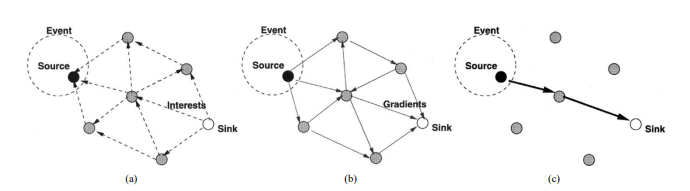
\includegraphics[width=1.0\linewidth]{figuras/roteamento orientado a dados.png} 
        \label{fig:roteamento roteamento orientado a dados}
        \\ \small Fonte: INTANAGONWIWAT; GOVINDAN; ESTRIN (2000).
    \end{figure}
\end{frame}